\documentclass[12pt]{article}
\usepackage[margin=1in]{geometry}

\usepackage{color} % for highlighting

\usepackage{wrapfig}
\usepackage{graphicx}
\graphicspath{ {figures/} }
\usepackage{float} % to force figures in specific place
\usepackage{array} % to make table row spacing better

\usepackage{enumerate}
\usepackage{enumitem}
\setlist{nolistsep}

\usepackage[numbers]{natbib} % for bib


\title{Understanding the Clinical Microbiome \\ Biological Engineering Thesis Proposal}

\author{Claire Duvallet}
\date{October 11, 2016}

\begin{document}



\maketitle
\newpage
\tableofcontents
\newpage
\begin{abstract}
In spite of the recent increase in research on the human 
microbiome, there is not a clear consensus on the relationship between 
human microbial communities and disease. Microbes colonize our entire bodies,
supplementing our body's functions, priming and training our immune 
systems, providing resistance to colonization 
by pathogens, and contributing to maintenance of health or progression of disease. 
However, major knowledge gaps exist in this field. 
The microbiota of certain body sites have been much less studied than others, and 
even the most extensively studied body sites lack a 
synthesized understanding of the clinical relevance of human-microbe associations. 
Additionally, translating microbial associations into biological hypotheses
remains challenging due to the lack of centralized tools and databases
for assigning biological meaning to groups of microbes.

This thesis will expand our understanding of the clinical microbiome in three ways.
First, I will characterize the relationships between the microbial communities
of the aerodigestive tract and their associations with clinical factors, 
increasing our basic understanding of this under-studied system.
Next, I will perform a meta-analysis of published case-control gut microbiome studies
across many disease states, synthesizing many existing studies by 
identifying consistent microbial markers of health and disease.
Finally, I will curate groups of biologically related microbes
to enable enrichment analyses and generalizable interpretations
of results from microbiome studies. 



\end{abstract}
\newpage

\section{Overall objectives and specific aims}
\subsection{Overall objectives}

The research presented in this thesis is united by a common purpose: 
advancing our understanding of the clinical human microbiome.
First, I will enrich our basic understanding of an under-studied 
microbial system by characterizing the relationships between the microbial communities
of the aerodigestive tract and their associations with clinical factors.
Second, I will synthesize results across many studies 
of a well-studied system, moving the field toward 
a better understanding of and consensus on the associations between 
gut microbial communities and human disease. To do this, I will perform a meta-analysis of 
published case-control gut microbiome studies
across many disease states to identify consistent microbial markers of health and disease.
Finally, I will curate
existing knowledge on microbial communities and develop a tool for 
inferring generalizable biological hypotheses from existing and future 
microbiome studies. 
Together, this work will contribute new knowledge
to the exciting field of human microbiome research and will 
empower researchers to draw clinically meaningful insights 
from their exisiting and future analyses.

\subsection{Specific Aims}
\begin{description}
	\item[Aim 1] Apply standard methods to identify microbial 
	community characteristics associated with gastro-esophogeal reflux 
	disease and aspiration.
	\begin{enumerate}
		\item Quantify relationships between lung, gastric, and throat microbial 
		communities.
		\item Identify clinical modulators of lung, gastric, and 
		throat microbial communities.
	\end{enumerate}
	\item[Aim 2] Perform a meta-analysis of gut 
	microbiome studies to identify consistent microbial signatures 
	within and across multiple diseases.
	\begin{enumerate}
		\item Compile and process publicly available case-control gut 
		microbiome studies with a standardized method.
		\item Determine whether certain microbes are consistently 
		associated disease in general or with specific diseases.
		\item Identify relationships between physiologically-related 
		diseases by comparing their microbial characteristics.
	\end{enumerate}
	\item[Aim 3] Enable generalizable interpretations of microbiome 
	analyses by assigning bacteria to groups with similar characteristics 
	and known associations with disease.
	\begin{enumerate}
		\item Combine existing databases with targeted literature searches 
		to define \textit{microbe sets} based on known biological 
		relationships.
		\item Use machine-learning techniques to extract disease-associated 
		\textit{microbe sets} from datasets collected in Aim 2.
		\item Develop these \textit{microbe sets} into a collaborative 
		tool for use in interpreting new microbiome studies.
	\end{enumerate}
\end{description}
\newpage

\section{Background and significance}

The topics addressed in this thesis are broad, and are all connected by
the motivation to better understand
clinically-relevant associations between microbes and their human hosts.
My work will focus on the microbial communities of two major body systems:
the aerodigestive and gastrointestinal tracts. To study these, I will 
use a combination of traditional analytical techniques, supplemented by 
novel methods as required. This section will provide background on
the aerodigestive tract, the gut microbiome, and current analytical techniques 
used in microbiome studies. 

\subsection{Aerodigestive tract}

\subsubsection{Physiology and disease}

\begin{itemize}
\item The aerodigestive tract is linked and the microbial exchange across
sites is unknown.
\item Gastro-esophogeal reflux disease (GERD) and aspiration are both complex and prevalent conditions that are thought to be related to respiratory diseases.
\end{itemize}

\begin{figure}[H]
%\begin{wrapfigure}{R}{0.2\textwidth}
\begin{center}
    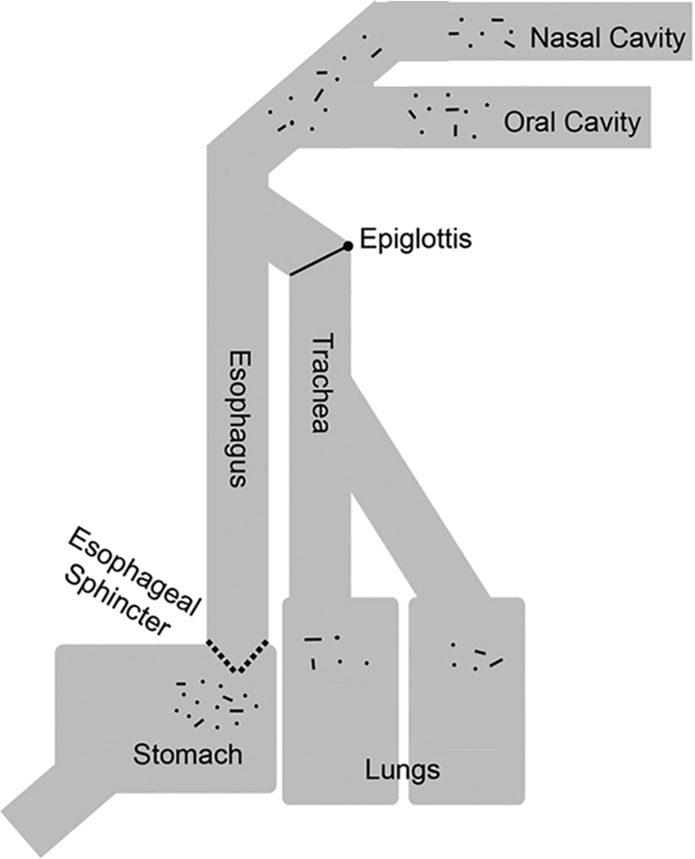
\includegraphics[scale=0.35]{aero_tract}
    \caption{Schematic of the flow relationship between sites of the 
    aerodigestive tract. Adapted from \cite{bassis-source-2015}.}\label{fig:aero_tract}
\end{center}
\end{figure}
%\end{wrapfigure}

\subsubsection{Microbiome of the aerodigestive tract}
\begin{itemize}
\item Lung and gastric microbiomes have historically been poorly studied. In the lung, a few diseases have been examined. In the stomach, it's mostly been related to \textit{H. pylori}.
\item The relationship between communities across the aerodigestive tract is still up for debate.
\end{itemize}

\subsection{Gut microbiome}

\subsubsection{Gut microbiome in health and disease}
\begin{itemize}
\item The gut is important to human health and disease, and gut microbes are important to the gut.
\item Lots of diseases have been hypothesized to be associated with the gut microbiome. Here's one or two sentences about IBD, CRC, and CDI.
\end{itemize}

\subsubsection{Existing understanding of the gut microbiome}

\begin{itemize}
\item It's been hard to find consensus on specific disease associations.
\item But we do know that the microbiome is stable and modifiable. People generally think that diversity and Bacteroides/Firmicutes ratios matter.
\item Existing meta-analyses haven't found much consensus either and they have focused on one or two diseases only.
\end{itemize}

\subsection{Analytical background and significance}

\subsubsection{Data generation, analysis and associated challenges} 

\begin{itemize}
\item Turning next generation 16S sequencing data into OTU tables is a process with lots of steps which are not standardized.
\item Resulting 16S data is hard to analyze because it is high-dimensional, sparse, and has lots of batch effects.
\item People find associations with disease by looking at alpha and beta diversity and doing univariate tests on OTU abundances.
\end{itemize}

\subsubsection{Interpreting taxonomy-based mmicrobiome analyses}\label{sec:gsea}
\begin{itemize}
\item When you do univariate analyses, you get a list of OTUs that are associated with the phenotype. Then it's up to you, the researcher, to figure out what those OTUs mean.
\item Enrichment analysis is a direct way to identify biologically meaningful patterns in data. It's been used in RNA data a lot (GSEA). 
\item For enrichment analyses to work, you need to have curated groups of related features (i.e. microbes). This doesn't really exist for microbes.
\end{itemize}

\section{Research design and methods}

The research presented in this thesis is united by a common purpose: 
advancing our understanding of the clinical human microbiome.
First, I will enrich our basic understanding of an under-studied 
microbial system. Second, I will collect and synthesize 
results from many studies of a well-studied system, to move the 
field toward a better understanding of the interactions between 
microbial communities and human disease. Finally, I will curate
existing knowledge on microbial communities to develop a tool for 
inferring generalizable biological hypotheses from existing and future microbiome studies.

\subsection{Aim 1: Aerodigestive microbiota associated with GERD and aspiration}

GERD, aspiration, and respiratory infections are three related
conditions with complex and unclear interactions.
We know that aspirating patients are at a higher risk for respiratory
infections, and that many patients who present with idiopathic
respiratory problems have a high prevlance of GERD. 
Furthermore, the microbial communities of the aerodigestive tract
are connected and likely exchange bacterial members, which may
contribute to respiratory infections. We hypothesize that the
microbial communities of the aerodigestive tract are extensively
exchanging microbes, and that certain clinical conditions like aspiration
or GERD may modulate the amount of exchange happening across various sites.

To address this hypothesis, we will first identify which microbes
are exchanged across sites and define a metric to quantify the ``extent'' of this exchange. 
To define this metric, we will incorporate both the co-occurence and the abundance
of microbes in the two sites and calculate it for each site-combination.
Next, we will identify clinical factors that have an effect on microbial
exchange in the aerodigestive tract. Specifically, we will investigate how aspiration,
reflux, and PPI use affects the similarity of communities and the
exchange of microbes between sites in the aerodigest tract.
We hypothesize that aspiration will increase the lung-throat connection and 
that reflux and PPI use will strengthen the stomach-lung connection.
Quantitatively describing the amount of microbial exchange happening in the
aerodigestive tract and determining clinical modulators of this exchange
will contribute new knowledge to our current understanding of the
aerodigestive microbiome, and could inform future aerodigestive
investigations and treatments.

\subsubsection{Aerodigestive patient cohort}

\begin{itemize}
\item Our cohort consists of 261 patients recruited by Rachel Rosen at Boston Children's over the past 6 years.
\item We have throat swabs, gastric fluid, and BAL. We also have aspiration and reflux metadata.
\end{itemize}

%\begin{wraptable}[H]{5.8cm}
\begin{table}[H]
\begin{center}

\begin{tabular}{l c}
	\hline
	\textbf{Sites} & \textbf{N} \\
	\hline
	gastric, throat, \& BAL & 87 \\
	gastric \& throat & 45 \\
	gastric \& BAL & 34 \\
	BAL \& throat & 9 \\
	\hline 
\end{tabular}
\end{center}
\caption{Samples in study}\label{tab:rosen_samples}
\end{table}
%\end{wraptable}

\subsubsection{Quantify exchange of microbes between lung, gastric, and throat communities} \label{sec:exchange}

\begin{itemize}
\item First, we'll define exchanged microbes and quantify them as the 
percentage of patients who are exchanging that microbe across their two sites ($p_s$), (Figure \ref{fig:sharedness_defn}).
\item It's possible that the gastric-lung exchanged microbes come from the environment, because of the low biomass of these sites. We'll look at them on a tree and in the literature to make sure that's not the case.
\end{itemize}

%\begin{wrapfigure}{R}{0.5\textwidth}
%	\centering
\begin{figure}[H]
\begin{center}
    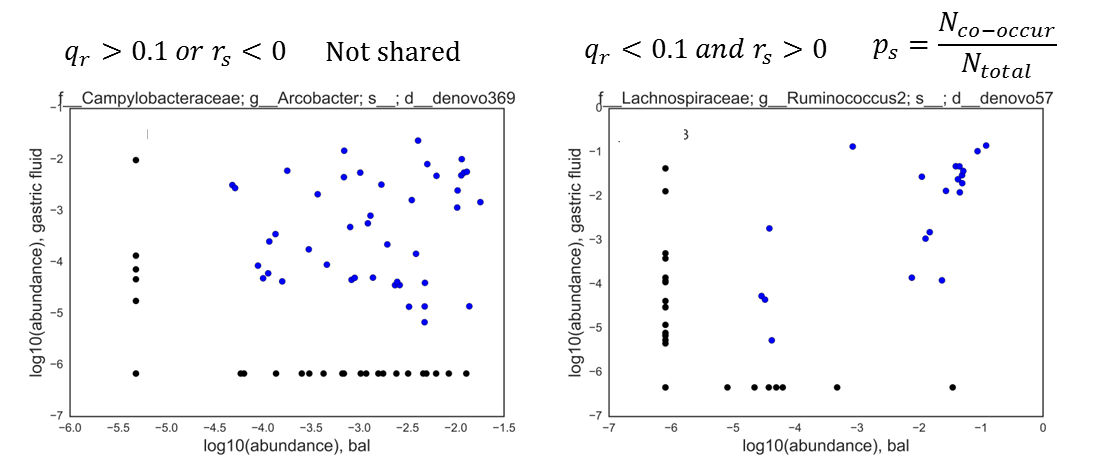
\includegraphics[scale=0.6]{sharedness_definition}
    \caption{If the abundance of a microbe when it is 
    present in both sites is correlated, then we consider it exchanged 
    across those sites (blue points, right panel). $p_s$ is then calculated as the 
    percentage of patients who have the microbe present in both sites (blue 
    points divided by total points, where each point represents one patient). 
    Example of microbes which are (A) not exchanged and (B) exchanged between stomach and lungs.}\label{fig:sharedness_defn}
\end{center}
\end{figure}
%\end{wrapfigure}

\subsubsection{Identify clinical modulators of lung, gastric, and throat microbial communities}

\begin{itemize}
\item We hypothesize that aspiration, reflux, and PPI use will affect exchange across sites. We'll calculate $p_s$ and look at beta diversity for the different groups.
\item We hypothesize that aspiration will modulate the 
amount of throat-lung and gastric-lung exchange, that reflux will modulate 
the amount of gastric-lung exchange, and that PPI use may also affect
the gastric-lung connection.
\item Some caveats to this work are that we're not really addressing directionality of the exchange and we don't have metadata on whether patients developed respiratory infections.
\end{itemize}

\subsection{Aim 2: Meta-analysis of gut microbiome studies}\label{sec:aim2}
By combining results from existing gut microbiome case-control 
studies, we can move the field toward a consolidated understanding of 
consistent microbial markers of gut-related diseases. We hypothesize 
that certain bacteria will often be associated with disease, and that 
some of these bacteria will be associated with many different types of 
diseases while others will be unique to one or two conditions. 
Additionally, we hypothesize that microbial signatures  of health and 
disease will be more similar in similar diseases (i.e. in diabetes and 
obesity vs. in diabetes and autism).

To address our hypotheses, we will first acquire a comprehensive
collection of case-control gut microbiome datasets and process them
with standardized methods. We will analyze each dataset individually
and synthesize the results from all datasets with basic meta-analysis 
techniques to identify microbes consistently associated with health or 
general disease. We will also perform a similar intra-disease meta-analysis 
for studies analyzing the same disease to identify microbes
that may be specific markers of certain disease and not others.
Finally, we will identify relationships between physiologically-related 
diseases by comparing their microbial characteristics across multiple
datasets. This comprehensive pan-disease meta-analysis will
consolidate the findings from many existing gut 16S microbiome studies,
synthesizing our existing knowledge and generating new hypotheses to
inform future mechanistic experiments and case-control analyses.

\subsubsection{Compile and process gut microbiome datasets}

\begin{itemize}
\item We'll collect and process all 16S case-control stool datasets that we can find through a standard pipeline.
\item We'll start our analyses by collapsing to genus level, but if that doesn't work we'll also look at higher-order taxonomic levels.
\end{itemize}

\subsubsection{Identify microbial markers of disease}\label{sec:indep_studies}

\begin{itemize}
\item We'll do univariate analyses on each dataset individually, and combine the results across \textit{all} datasets using a modified Fisher's method for combining p-values.
\item Next, we'll do an intra-disease meta-analysis, combining results from datasets looking at the same disease. We hope to find microbes that are associated with a specific disease but not with disease in general, or that have a different directionality of association.
\item We might not be able to find anything, probably because of batch effects. Developing robust methods to overcome technical batch effects in 16S 
studies is not within the scope of this work, but there are many
simpler options available to help mitigate severe batch effects.
\end{itemize}

\subsubsection{Compare results between studies for related diseases}\label{sec:signatures}
\begin{itemize}
\item Our next hypothesis is that similar diseases will have similar 
signatures of dysbiosis. We'll summarize each dataset with a ``microbial signature'' and see which datasets/diseases cluster together.
\item We expect diseases with strong microbiome associations to cluster together. We may also see diseases with similar underlying causes (i.e. inflammation) clustering together (Figure \ref{fig:microbe_signatures}).
\end{itemize}


%\begin{wrapfigure}{R}{0.5\textwidth}
%	\centering
\begin{figure}[H]
\begin{center}
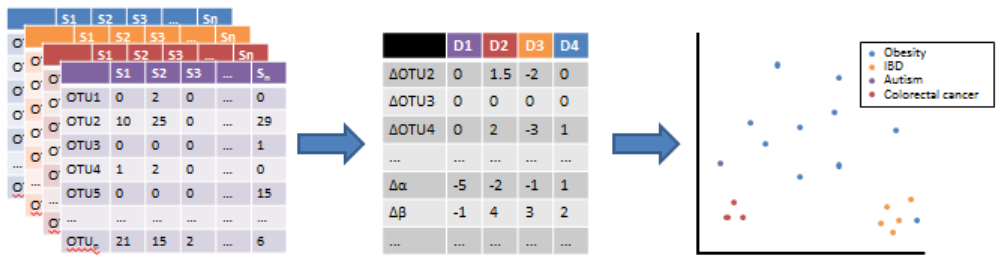
\includegraphics[scale=0.5]{microbial_signatures}
\caption{Defining microbial signatures}\label{fig:microbe_signatures}
\end{center}
\end{figure}
%    \caption{Defining microbial signatures}
%\label{fig:microbe_signatures}
%\end{wrapfigure}

\subsection{Aim 3: Assigning bacteria to groups with similar functions and disease associations}

In this aim, we will curate biologically-motivated \textit{microbe 
sets} to enable easier interpretation of results from 16S microbiome 
analyses. By defining groups of related microbes, we 
will enable enrichment analyses like GSEA, but for microbiome data (Section \ref{sec:gsea}). Enrichment analyses will allow for better 
biological understanding of results from individual studies as well as 
more consistent comparisons of results across studies reported in 
the literature.

To define \textit{microbe sets} that facilitate enrichment analyses, we will
begin by searching the literature for existing microbial annotation
databases and papers which characterize broad groups of microbes.
In parallel, we will also mine the datasets and results from Aim 2
for meaningful microbial associations with human phenotypes such as
disease or inflammation (Figure \ref{fig:microbe_sets}). Finally, we will combine and package this information
in a format that is easy to use and update as future studies contribute
to the field. This tool will enable future microbiome scientists to extract more
meaningful information from their microbiome studies, thus
contributing significantly to increasing our understanding of the
clinical and scientific relevance of the human microbiome.

\begin{figure}[H]
\begin{center}
	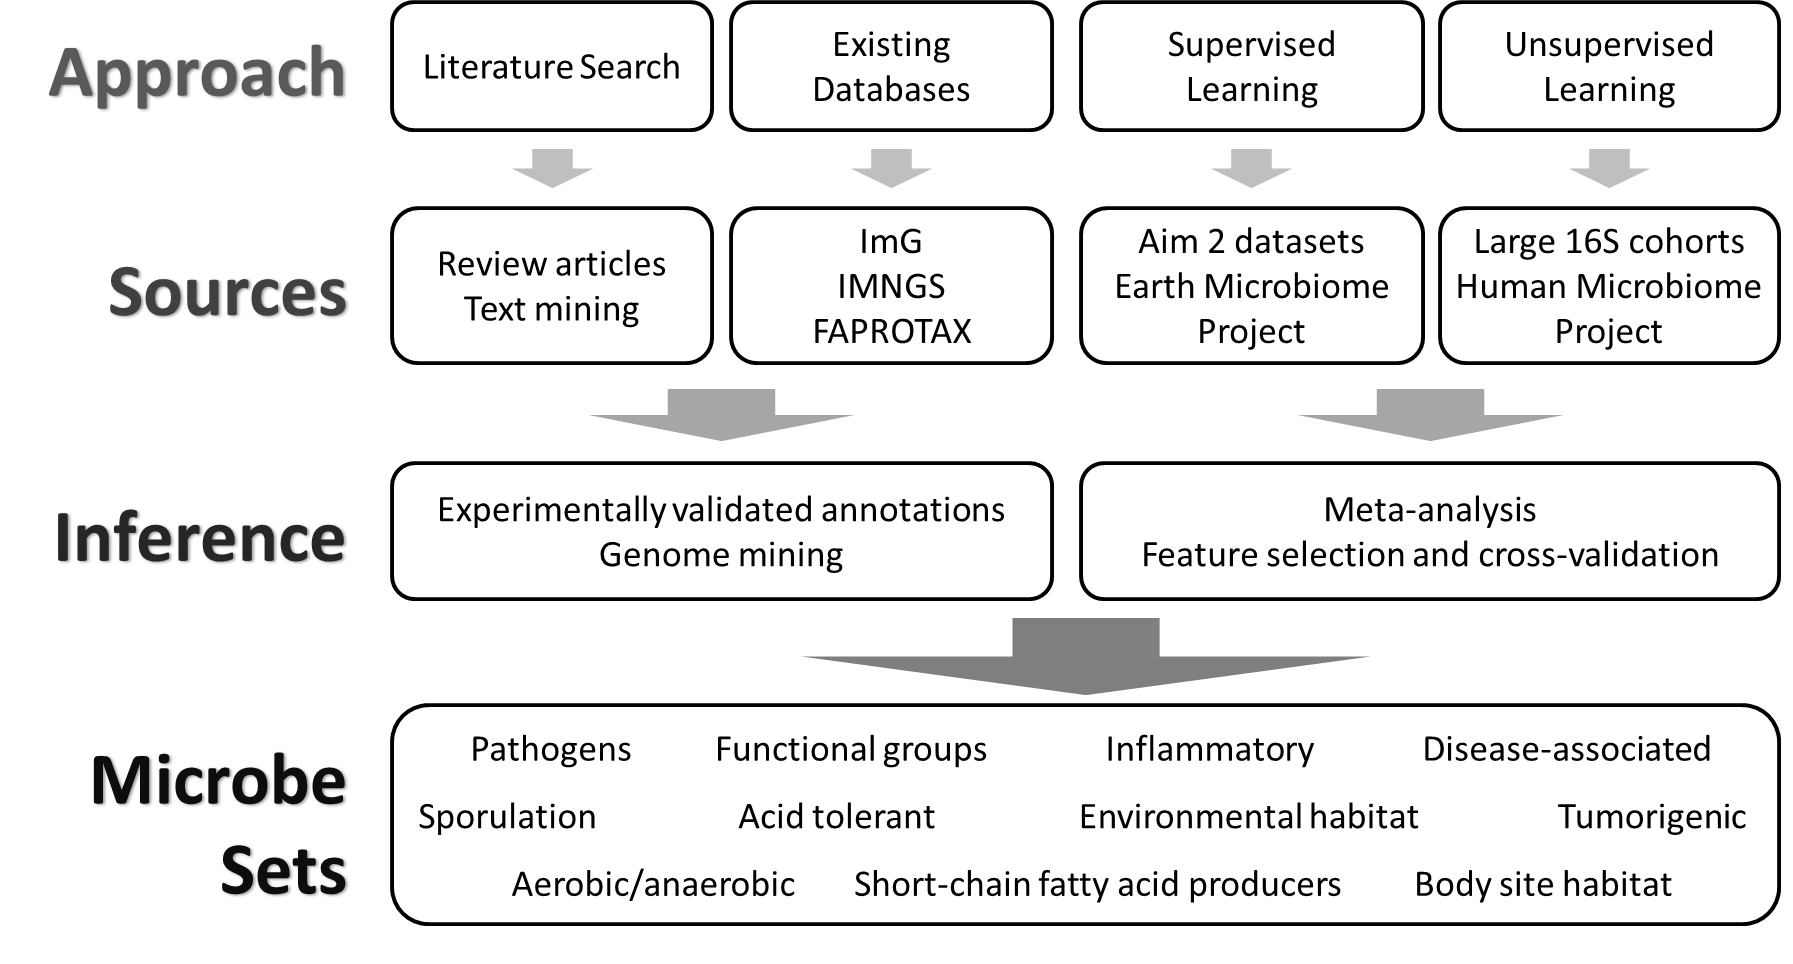
\includegraphics[scale=0.5]{microbe_sets}
	\caption{A variety of approaches will be used to define
	microbe sets, including manual curation from literature
	and database searches and data-driven methods (``Approach'').
	Many different kinds of resources will be drawn upon 
	(``Sources'') to infer groups of related microbes 
	(``Inference'') based on different categories 
	(``Microbe Sets'').}
	\label{fig:microbe_sets}
\end{center}
\end{figure}


\subsubsection{Define microbe sets based on known biological relationships}

\begin{itemize}
\item We'll start with a literature and database search to see what's out there in terms 
of microbial annotations. We'll start with the ImG database and see what's in it and 
what needs to be filled out.
\item In collboration with Ilana, we'll do a combination of literature mining and 
bioinformatics inference to fill out our annotations.
\item We'll also build a tree from the 16S sequences of all the bacteria we annotate and 
maybe do some phylogenetic inference to fill out more annotations.
\end{itemize}

\subsubsection{Extract disease-associated microbe sets from datasets in Aim 2}

\begin{itemize}
\item We'll also define some microbe sets based on the results from meta-analyses in Aim 2, and from machine-learning magic on the datasets from Aim 2 (Table \ref{tab:classifications}).
\item The machine-learning stuff may not work so we'll try a few other approaches. 
\end{itemize}

{
\renewcommand{\arraystretch}{1.2}
\begin{table}[H]
\begin{center}
\begin{tabular}{ m{6cm} m{10cm} }
	\hline
	\textbf{Microbe set association} & \textbf{Classification task} \\
	\hline
	General health/disease & All healthy vs. all disease \\
	%\hline
	Diarrhea & CDI, EDD, IBS-D vs. controls \\
	%\hline
	Neurological & Autism, Parkinson's vs. controls \\
	%\hline
	Liver & NASH, MHE vs. controls\\
	%\hline
	Metabolic syndrome & T1D, T2D, obesity, metabolic syndrome vs. 
	controls \\
	%\hline
	Autoimmune/inflammatory & T1D, rheumatoid arthritis, psoriatic arthritis, Crohn's disease 
	vs. controls or non-autoimmune patients \\
	\hline
\end{tabular}
\caption{Classification tasks to identify groups of phenotype-associated microbes}\label{tab:classifications}
\end{center}
\end{table}
}

\subsubsection{Develop collaborative tool for interpreting microbiome studies}
\begin{itemize}
\item We'll make our annotated microbe sets available to researchers and will build a 
tool that does the enrichment analyses on their data for them.
\item This is going to be hard and it's okay if it's not perfect or comprehensive
because it's mainly going to be used as a hypothesis-generation tool.
\end{itemize}

\section{Preliminary studies}

\subsection{Aim 1}
\subsubsection{Microbiome community exchange}

\begin{itemize}
\item We found a lot of exchanged microbes, the majority of which were between the throat and stomach (as expected). 
\item Interestingly, we also found lots of exchange/similarity between the stomach and lungs. This might have to do with microaspiration of gastric contents. 
\end{itemize}

\subsubsection{Modulators of community exchange}

\begin{itemize}
\item We found that aspirators share more between and have more similar throat and lung communities than non-aspirators.
\item Our first pass with reflux showed that there might be more stomach-lung exchange 
in patients with more frequent full-column reflux. Interestingly, this wasn't reflected 
in the ``exchanged microbes'' but rather in the beta-diversity of stomach and lung 
communities, indicating that the exchange might be more stochastic here.
\end{itemize}

\subsection{Aim 2}
\subsubsection{Collecting and reprocessing 16S case-control datasets}

\begin{itemize}
\item We've collected and processed about 30 datasets. These are summarized in 
a table that I still need to compile (N patients, sequencing depth, sequencing technology).
\end{itemize}

\subsubsection{Identify general patterns of health and diseases}

\begin{itemize}
\item First we looked at alpha diversity, and saw that it was only consistently 
different in diarrheal diseases.
\item Then we did univariate analyses for each study. Looking at the pattern, we noticed 
that diarrheal diseases have broad community shifts. The other diseases are less clear.
\item We also did the Fisher's method for combining p-values. Results from this 
are TBD this weekend. I think we'll find a handful of genera that are significantly
associated with health or disease when we combine *all* diseases together.
\end{itemize}


\bibliographystyle{unsrtnat}
\bibliography{refs}

\end{document}